%% XXX This is not content!! XXX
%% Your content is in 'content.tex'.

\newcommand{\ssaroot}[1]{../../#1}
\documentclass{\ssaroot{svmono}}
\ssainput{headers}{packages.tex}
\ssainput{headers}{style.tex}
\ssainput{headers}{macros.tex}
}

% disable index command when generating tikz figures
\ifthenelse{\equal{\jobname}{\detokenize{chapter}}}{
  \message{Compiling regular chapter^^J}
}{
  \message{Compiling figure \jobname^^J}
  \def\index#1{}
  \def\printindex{}
}

\pgfrealjobname{chapter}


% =========================================================
% Set the page headers to show the date and time
\pagestyle{fancy}
\lhead{\today}
\rhead{\currenttime}

\fancypagestyle{plain}
{
	\lhead{\today}
	\rhead{\currenttime}
}
% =========================================================

\makeindex

\begin{document}

\listoftodos

	\chapter{if conversion \Author{C. Bruel}}
\inputprogress
\graphicspath{{img/}{if_conversion/img/}{part4/if_conversion/img/}}
	
\newcommand\cond{~?~}

%\setcounter{tocdepth}{3} 
%\tableofcontents

\section{Overview/Motivations}

We describe in this chapter an if-conversion algorithm in SSA representation. If-conversion is the process by which a control flow region is optimized into an equivalent region were branches have been removed. We start with a description a full SSA model, taking as input a SSA region and produces a SSA region using speculation. We then describe how this framework is extended to use predicated execution, using the $\psi$-SSA presented in chapter ???. 

\subsection{Introduction}

A way to increase the instruction throughput is to increase the IPC (number of instrucion per cycle), either by increasing pipeline depth, or by increasing the number of instructions that are excecuted simultaneously. This can be achieved by multiple issue processors. Out-or-order expensive superscalar execution models use dynamic scheduling. In-order execution model, becoming popular because lower hardware complexity and delegate to the compiler or to the programmer the responsibility to organize the parallel execution of the execution flow \cite{Rau:2003:IP:1074100.1074489}.

In order for the compiler to organize the parallelism explicitly, VLIW (Very Large Instruction World) or EPIC (Explicitly Parallel Architectures) make the parallelism visible to the ISA representation, allowing a static scheduler to organize the assembler such as a maximum number of instructions are issued for each cycle. 

Unfortunately, programs contains many sequences of instructions that can't be parallelized, because of control or data dependencies. Different Instruction Level Parallelism techniques are implemented in the hardware, such as dynamic scheduling, branch prediction, or in the compiler, such as software pipeline, vectorization or loop optimizations. But still, despite those efforts, the execution flow is still disrupted by conditional branches, and many ALU cycles are wasted. ILP was proved to be very effective to extract performances in the mathematical fields for evaluation of polynomial expressions \cite{Jeannerod:2010:TTI:1837210.1837212}, embedded processor rely on ILP to sustain performance required for multimedia applications \cite{FisherFaraboshiYoung} and even general purpose processor, or more scalar applications benefits from this optimization.

Conditional branches introduce control dependencies between instructions. An instruction is control dependent on a preceding instruction if the first one determines the execution of the second one \cite{Kennedy:2001:OCM:502981}. They limit the scope of ILP optimizations, because they reduce the number of continuous instructions that are not data dependent and thus can be executed in parallel. By reducing the average size of a basic block, they act as a bottleneck for exposing parallelism.

If-conversion is the process of transforming a control flow region containing a several basic blocks into a single basic block of straight line of conditional instructions. Thus removing control branches from this region \cite{Schlansker97achievinghigh}. The conditional instructions are implemented on the target machine using the predication or speculation techniques described bellow. 

Removing branches improves performance in several ways: by removing the mis-prediction penalty, the instruction fetch throughput is increased and the instruction cache miss penalty reduced. Enlarging the size of the basic blocks allows the static scheduler to schedule earlier long latencies operations and to improve the ILP by merging multiple control paths into a single flows of execution. Many compiler optimizations are impacted by branches. Software Pipelining for example, can't efficiently schedule loops with conditional branches \cite{Warter:1992:EMS:144953.145796}.

Consider the simple example \ref{fig:example1}, that represents the execution of a double if-then-else statement on a hypothetical 3-issue processor. Branches are not highly biased, so the minimal schedule height is 3 instructions (assuming a fallthru is free), and the maximal schedule height is 5 instructions.

\begin{figure}
  \subfloat[Control Flow] {
    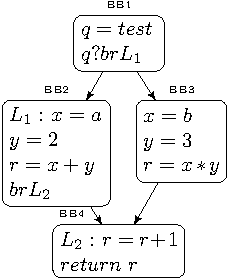
\includegraphics{specul}
    \label{fig:orig}}
  \subfloat[After if-conversion using conditional moves] {
    \begin{tabular}{|l|l|l|}
     \hline
       ALU1 &  ALU2 &  ALU3  \\
     \hline
      $q = test$ & $p = test$ & $x1=a$ \\
      $y1=x$      & $y2=3$      & $x2=2$ \\
      $x=q?x1:x2$ & $y=p?y1:y2$ & \\
    \end{tabular}
    \label{fig:specul}}
\caption{I don't like this Example, change for a 4-issues}
\label{fig:example1}
\end{figure}

After if-conversion the execution path is reduced to 3 cycles, regardless of the tests outcomes. 

We can observe here that if-conversion implied two beneficial transformations.
\begin{itemize}
\item  Merge of execution paths into a single execution path, implying a  better exploitation of available resources.  
\item Reduction of the schedule length, because instructions can be speculated before the branch.
\end{itemize}

This simple introductory example already instructs us that:

\begin{itemize}
\item Variables need to be renamed, 
\item a \textit{merge} pseudo operation have been introduced. It is necessary to reconstruct the original value of $x$ and $y$.
\item This \textit{merge} introduces a data dependency. if-conversion transforms control dependencies into data dependencies \cite{Allen:1983:CCD:567067.567085}. 
\end{itemize}
This looks like very much SSA ! considering that the merging point can be materialized into the original control flow by the $\phi$ pseudo operation.

\subsection{Architectural requirements}
The example illustrates that if-conversion's output needs some conditional form of execution on the target's architecture. Depending on the available support, the algorithm must be able to match the ISA, to provide support for conditional execution of instructions, or to conditionally commit the result of an instruction.
Basically, several kind of support for predication can (co-)exist: predicated execution  or speculative execution my mean of conditional moves. The partially predication model predicates subset of the ISA, for example the load and stores that are difficult to speculate.

Predication is an architectural feature that allows an instruction to be executed conditionally by mean of a predicate.

\begin{figure}
\begin{minipage}[t]{3cm}
\mbox{fully predicated} \\
$ p \cond x = a + b $ \\
$ \overline{p} \cond x = 0 $ \\
\end{minipage}
\begin{minipage}[t]{3cm}
\mbox{select} \\
$t = a + b $ \\
$x= p \cond t : 0 $ \\
\end{minipage}
\begin{minipage}[t]{3cm}
\mbox{cmov} \\
$t = a + b $ \\
$x = 0 $ \\
$x = cmoveq$ $t$ \\
\end{minipage}
\caption{Conditional execution using different models}
\label{fig:pred}
\end{figure}

Speculation is a compiler technique that allows instructions that are control dependent to be executed unconditionally. The result can be committed only when the condition is known to be true. Examples of conditional moves are the $cmov$ (Pentium Pro) or the $select$ (ST 231 VLIW) instructions.

Example \ref{fig:pred} shows a conditional execution using the different modes.

To be speculated, an instruction should not potientially create any other side effects, or hazards. For instance a memory load should not trap (cache misses can also be considered for performance). This of course prevents unconditional execution by mean of speculation of memory access for which the address is valid only on the selected path. unless the is architectural supports to dismiss bad memory access errors. Examples are the $ldw.d$ dismissible load operation for the $ST231$ processor or ... ? 
Speculative load is important. First programs usually contains a large number of memory operations, so not being able to speculate them would block almost all oportunities for if-conversion. Second as a long latency operations, the data can be fetched higher in the instruction stream, reducing stalls.
Speculative stores can be performed on speculating the address value, and forcing it to be a dummy valid address in case of not taken path.

\begin{figure}
\begin{minipage}[t]{4cm}
\mbox{speculative load:} \\
$t = ldw.d(addr) $ \\
$x = select p \cond t : 0 $ \\
\end{minipage}
\begin{minipage}[t]{4cm}
\mbox{speculative store} \\
$x=select p \cond addr : dummy $ \\
$stw (x, value) $
\end{minipage}
\label{fig:spec}
\end{figure}

The condition code must be visible at the ISA level, to enable boolean optimization of predicates.

\section{SSA if-conversion}

SSA provides an efficient intermediate representation in which false data dependencies have been removed, removing the need for register renaming when merging two definitions into one. Each assignment target (def) is assigned a unique register name. Registers are re-materialized at join nodes using $\phi$ operations. A procedure is in minimal SSA form if the number of $\phi$ instructions at join nodes is as small as possible. In relation to the if-conversion, SSA-form representation ensures that a variable is assigned only once, and their merging point is exposed info $\phi$ operations.

General steps for if-conversion.

\begin{itemize}
\item Multiple definitions of a different variables assignment merged into a single path. This is inherently fixed in SSA, alleviating the need for renaming.
\item Minimize the number of instructions to be predicated. Only instruction that merge need to be conditioned inside the predicate set that control the merge. Others can be safely executed when they don't produce hazard. 
\item Predicate assignments. Each instruction in the basic block that merge into the $\phi$ must be assigned to their defining predicate
\end {itemize}

Finally the conditionalized instructions must be emitted. in \ref{fig:nested1}, instructions from BB2 are assigned with the predicate $p$ and instructions from BB3 with the predicate computed from $q\&t$. \ref{fig:nested2} shows the code layout after predicate assignments. Then, In case of speculation execution model, predicated instructions have to be converted into conditional moves, using temporaries to hold arithmetic values. Additionally, a new predicate will need to be computed and assigned to each instruction.

\begin{figure}
\centering
  \subfloat[Nested test] {
    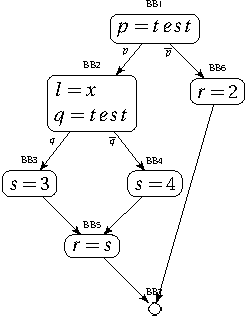
\includegraphics[scale=0.9]{nested1}
    \label{fig:nested1}}
  \subfloat[Predicate Assignments] {
    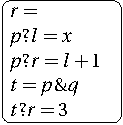
\includegraphics[scale=0.9]{nested2}
    \label{fig:nested2}}
  \subfloat[Conversion to speculated] {
    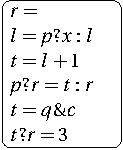
\includegraphics[scale=0.9]{nested3}
    \label{fig:nested}}
\caption{Traditional support for partial predication}
\label{fig:trad_part_pred}
\end{figure}

In contrast, consider the equivalent SSA if-conversion in \ref{fig:nest_ssa}, speculation is the genuine way of producing conditional moves out of $\phi$ instructions. Predicates don't need to be computed and temporaries values don't need to be conditioned. As a result the SSA aggressive speculation technique produces a schedule length of 3. While traditional support produces in this case a schedule length of 4, without further expensive predicate reduction optimization.

\begin{figure}
\centering
  \subfloat[Nested test] {
    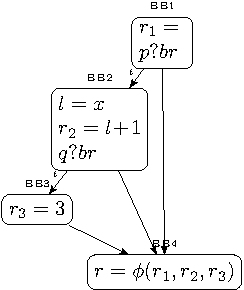
\includegraphics[scale=0.9]{nested4}
    \label{fig:nested4}}
  \subfloat[Inner if-conversion] {
    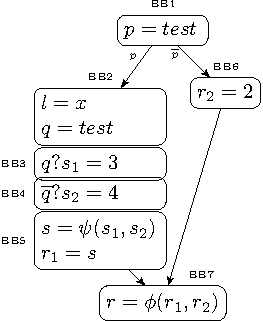
\includegraphics[scale=0.9]{nested5}
    \label{fig:nested5}}
  \subfloat[Global if-conversion] {
    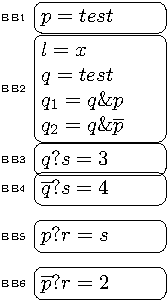
\includegraphics[scale=0.9]{nested6}
    \label{fig:nested6}}
\caption{SSA-based partial predication}
\label{fig:nest_ssa}
\end{figure}
Note that basically, Since a SSA $\phi$ express the merging point of $n$ definitions from $n$ predecessors, the definition points depends on their nearest condition under which they depend. Intuitively we already know that thanks to SSA the definition point is straightforward to find, since it corresponds to the path by which the $\phi$ operand is reached. 
A very big difference in nature is in the way the merging of conditional is realized using data dependencies instead of predicate selection. In SSA the condition merge assignment is not realized thru $\&$ if predicates, but using two successive conditional moves operations.

This algorithm takes as input a structured region in pure SSA form and produces a pure SSA using conditional move instructions to realize join points. One benefit of this approach is that all SSA properties are maintained, and scalar optimizations, such as constant propagation can be executed without predicate awareness.

\subsection{SSA operations on basic blocks}

SSA if-conversion works iteratively from inner regions to outer regions, using a set of transformations on conditional branches that we describe here.

\begin{figure}
  \subfloat[phi removal] {
  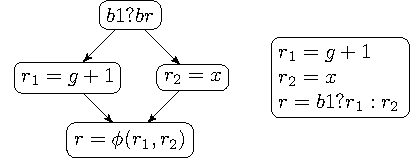
\includegraphics[scale=0.8]{phi_removal}
  \label{fig:phi_rem}}
  \subfloat[phi reduction] {
  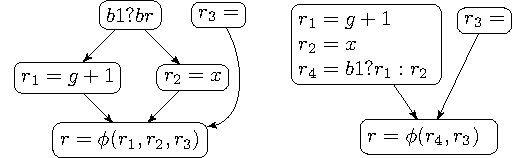
\includegraphics[scale=0.8]{phi_reduction}
  \label{fig:phi_red}}
  \subfloat[phi augmentation] {
  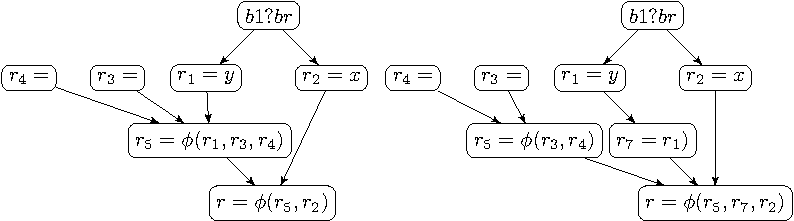
\includegraphics[scale=0.8]{phi_augmentation}
  \label{fig:phi_aug}}
\label{fig: phi_operations}
\end{figure}

The basic control structures that the analysis recognizes is the Single Exit region formed from the minimal set of blocks between a branch point and a merge point.  Those are minimal single entry single exit regions because at this point nested regions were already if-converted.

 We define this structure as the region between a conditional block and the first common immediate post-dominator of the taken path block and the fall-thru block.

Note that each path can contain zero or more basic blocks with incoming edges.

We allow two successive conditional blocks sharing one immediate post-dominator to be merged with logical operations after a normalization transformation. The normalization transformation ensures that conditional blocks sharing a same target can be merged by defining a wired $or$, or a wired $and$ share the same branch characteristics using branch reordering, test inversion or $de-morgan$ transformations.

\begin{figure}
  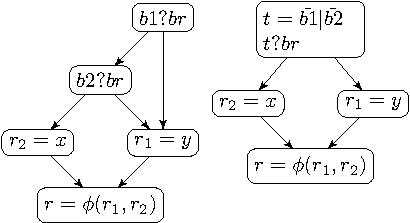
\includegraphics[scale=0.8]{phi_merge}
  \label{fig:phi_merge}
\end{figure}

Consider a conditional branch depending on a predicate $p$ and a region starting at $BBhead$. Let $BBp$ be the set of single exit basic blocks $(BBi,\dots,BB_n)$ that are on the taken path if $p$ is true and $BBq$ be the set of single exit basic blocks $(BBj,\dots,BB_m)$ that are executed if $p$ is false. The merge point of the if-converted region is at $BBjoin$. We distinct 4 types of basic SSA transformation that the framework uses and produces:
\subsubsection{$\phi$ removal} (figure \ref{fig:phi_rem})
The join node of the considered region has two predecessors and $\phi$ instructions are of the form $r=\phi(r_1,r_2)$. After speculation of the definitions of $r_1$ and $r_2$ the instruction can be rewritten as $r=\psi(p?r_1,\overline{p}?r_2)$.
% \begin{proof} Once $BBp$ and $BBq$ have been promoted into $BBhead$, $BBjoin$ has for only predecessor $BBhead$ so it is not in its dominance frontier. The $\phi$ is not necessary and is removed.
% \end{proof}
\subsubsection{$\phi$ reduction} (figure \ref{fig:phi_red})
 The join node of the considered region has $n$ predecessors that have $\phi$ instructions of the form $r=\phi(r_1,r_i,r_j,\dots,r_n)$. After merging, the $\phi$s are rewritten $t=\psi(p?r_i,\overline{p}?r_j)$ and a new $\phi$ $r=\phi(r_1,t,\dots,r_{n-1})$ is created with one operand less. The $\psi$ instruction is inserted after the speculated $r_i$ and $r_j$ definitions into $BBhead$.
% \begin{proof} $BBjoin$ is still in the dominance frontier of $BBhead$, A $\phi$ must be redefined with the new definitions. The two corresponding $\phi$ edges from $BBq$ and $BBp$ can be replaced by the $BBhead$ edge.
The join block $E$ has $n$ predecessors with $n > 2$, and $n$ blocks in its dominance frontier if it contains $\phi$s.
% \end{proof}
\subsubsection{$\phi$ augmentation} (figure \ref{fig:phi_aug})
The objective is to remove incoming edges into the region. 
Consider a join node with $n$ predecessors among which $p$ is duplicated into $q$.  The join node of the considered region have $\phi$ instructions of the form $r=\phi(r_1,p,r_i,r_j,\dots,r_{n-1})$. The instruction is rewritten $t=select(p,r_i,r_j)$ and \mbox{$r=\phi(r_1,t,q,\dots,r_n)$}. 
% \begin{proof}The duplicated blocks are new dominators of $BBjoin$ that define new $defs$. These blocks are now in the dominance frontier of $BBjoin$. SSA is maintained with new $\phi$ upgraded with the new reaching points.
Since the algorithm works the control flow in post order mode, the dominator tree doesn't change, and it's possible to maintain the SSA locally to the inner region. By recurrence the if-converted region can be in turn be optimized out if it's head belongs to the dominance frontier of an outer region.
% \end{proof}
Note that block duplication doesn't necessary implies more code size, since data flow dependencies are broken, new opportunities for propagation or scalar optimization arise. Here the local $t$ appears temporary, since $r2$ can be propagated into the $\phi$.

\subsection{SSA representation of conditional instructions}

One problem of the described SSA-speculative framework is that it doesn't fit very well with a predicated model of conditional execution. Since $\phi$ are transformed to realize joint points into conditional moves, we should backwalk to relink the conditional moves into predicated instructions. This process of transforming speculation into predication is not convenient for many reasons:
- Predication introduces a renaming problem: Since a same register name can have 2 different assignments (under different predicates), this breaks SSA rules. The solution is to re-use the framework to realize join points into an extended SSA representation:

In \cite{Stoutchinin:2001:ESS:563998.564022} $\psi$-SSA was described as a way to express a predicated form of SSA extension. Such representation is usually built from already predicated code, non SSA, originating from inlined assembly, peepholes, intrinsics functions or local transformations of control flow idioms. 

$\psi$-SSA expose the edge dependency from the basic block into which the definition of the $\phi$ argument is defined in the original CFG by a new data dependency. This dependency needs to be materialized into a $select$ or $\psi$ operation. Note that the $select$ operation is a real instruction that don't need to be replaced by the out-of-ssa process. If the target architecture doesn't provide such instruction to switch between speculated instruction, it can be emulated using two conditional moves. One advantage to generate $select$ instruction at this stage is that the program stays in full SSA form and make all the data dependencies explicit, and can be feed to all SSA optimizers. 

\begin{figure}
\begin{minipage}[t]{4cm}
\mbox{SSA:} \\
$ if (p) $ \\
$   x_1 = a+b $ \\
$ else $ \\
$   x_2 = 0 $ \\
$ x = \phi (x_1, x_2) $ \\
\end{minipage}
\begin{minipage}[t]{4cm}
\mbox{SSA-speculative form:} \\
$x_1 = a + b $ \\
$x_2 = 0 $ \\
$x = p \cond  x_1 : x_2$ \\
\end{minipage}
\begin{minipage}[t]{4cm}
\mbox{$\psi$-SSA form:} \\
$x_1 = a + b $ \\
$x_2 = 0 $\\
$x = \psi (p \cond x_1, \overline{p} x_2) $ \\
\end{minipage}
\end{figure}

Note that unlike $\phi$ arguments that are executed simultaneously (they don't depend each other), $\psi$ arguments are executed sequentially and ordered from their definition predicate set. This propriety is necessary because if-conversion replaces the ``spacial'' dependency from the CFG by a ``temporal'' dependency from the straight line predicated code.

The basic idea behind the SSA transformations is to replace $\phi$ operations by predicated instructions merging into a $\psi$ or speculated instructions merging into a $select$ equivalent instructions, while maintaining the SSA properties.

\subsection{SSA promotion}

To know the values that need to be conditionally defined, we only need to look at the defining instructions of the $\phi$ instructions. By elimination, all temporaries that do not have a join point into the considered region and that don't have a side effect are unconditionally speculated during the SSA transformations processes. Instructions with a side effect will need to be guarded. This is a considerable advantage over traditional if-conversion algorithms that marks all instructions in a conditional basic block as dependent on the predicate. By removing this predicate dependency, which is a data dependency, the instruction can be moved before the predicate assignment.

Our algorithm is applied iteratively on a control flow in SSA form until no more reductions are possible. The quality of the SSA taken as input does not affect the correctness of the algorithm: if the control flow is in pruned SSA, i.e two paths $x->+z$ and $y->+z$ converge at node z, then a $\phi$ node is inserted at z only if z is alive in or after z. if which case x and y are promoted and no $select$ operation is generated. if the SSA is minimal, a $select$ instruction would be generated and removed by dead code. Inserting dead code from minimal SSA only introduces noise in the local scheduling heuristics because of the false data dependencies.

\subsubsection{Partial redefinition}

A $\psi$ operation exposes new data dependencies, by expressing the merge of two definitions. Note that the order of the partial definition is important, so a definition partially redefines the preceding ones. We use this propriety to speculate the first definitions, so it becomes speculated instead of disjoint. This local optimization allow to remove a predicate dependency but also creates a new partial dependency (predicates are not disjoint). 

\begin{figure}
\footnotesize
\begin{minipage}
$ p = test $ \\
$ p \cond x_1 = a + b $ \\
$ \overline{p} \cond x_2 = c $ \\
$ x = \psi(p \cond x_1, \overline{p} \cond x_2) $ \\
\caption{disjoint predicates}
\end{figure}
\end{minipage}
\begin{minipage}
$ x_1 = a + b $ \\
$ p = test $ \\
$ \overline{p} \cond x_2 = c $ \\
$ x = \psi(T \cond x_1, \overline{p} \cond x_2) $ \\
\caption{optimized order predicates}
\end{minipage}
\end{figure}

$T$ represents the $True$ predicate. This optimization is useful to save one predicate register and to remove a data dependency between a predicate definition in its use. 
The $\psi$ definition is defined on the $T$ predicate set, therefore it is speculable, as shown here:

\subsubsection{$\psi$ speculation properties}

Since the algorithm processed the regions from inner to outer scopes, conditional operations will be in turn speculated or conditioned with a new condition. We define here $\psi$ operand promotion rules.

Consider the code \ref{fig:nested_psi} containing a subregion already processed. The $\psi$ operation can be safely speculated, since it's definition predicate domain is always true for $c$. Thefore the $\psi$ operation can become unconditionally executed, knowing that the nested condition level will be catched in the second $\psi$ in \ref{fig:nested_psi_speculated}.

\subsubsection{$\psi$ predication properties}

If the instructions are not speculable, then they must be predicated:
In \ref{fig:nested_psi_predicated}, the $c$ condition merges with all conditions under which the $\psi$ operands are defined. Here a new predicated $p_1$ is created to hold the predicate definition for the instructions defined under $c$. 

Note that conceptually, the speculative $\psi$ execution allows a predicate definition domain larger that the original one, which the predicative transformation exactly matches the initial definition domain, at the expense of for data dependencies and predicate computation.

We can see with this example that the decision to speculate or predicate can be done at the level of each joining definition, allowing a mix of them in the final program. The advantage to speculation over predication is a reduced dependency length. The disadvantage of speculation is that it increases register pressure until the merge point, and put long latencies operations on the critical path.
 
\begin{figure}
\footnotesize
\begin{minipage}[b]{4cm}
$ if (c) $ \\
$ \{ $ \\
\hspace*{2mm}$ x_1 = a + b $ \\
\hspace*{2mm}$ \overline{p} \cond x_2 = c $ \\
\hspace*{2mm}$ x = \psi(T \cond x_1, \overline{p} \cond x_2) $ \\
\hspace*{2mm}$ d_1 = use (x) $ \\
$ \} $ \\
$ else $ \\
\hspace*{2mm}$ d_2 = 3 $ \\
$ d = \phi(d_1,d_2) $ \\
\caption{nested if}
\label{fig:nested_psi}
\end{minipage}
\begin{minipage}[b]{4cm}
$ x_1 = a + b $ \\
$ \overline{p} \cond x_2 = c $ \\
$ x = \psi(T \cond x_1, \overline{p} \cond x_2) $ \\
$ d_1 = use (x) $ \\
$ \overline{c} \cond d_2 = 3 $ \\
$ d = \psi(T \cond d_1, \overline{c} \cond d_2) $ \\
\caption{speculated nested if}
\label{fig:nested_psi_speculated}
\end{minipage}
\begin{minipage}[b]{4cm}
$ p_1 = \overline{p} \& {c} $ \\
$ c \cond x_1 = a + b $ \\
$ p_1 \cond x_2 = c $ \\
$ x = \psi(c \cond x_1, p_1 \cond x_2) $ \\
$ d_1 = use (x) $ \\
$ \overline{c} \cond d_2 = 3 $ \\
$ d = \psi(T \cond d_1, \overline{c} \cond d_2) $ \\
\caption{predicated nested if}
\label{fig:nested_psi_predicated}
\end{minipage}
\end{figure}

\subsubsection{Predicate merging}

During the regions formation, subregions containing a block that is reached from two conditions can be optimized by merging predicates. A new predicate is computed using a logical operation on both basic blocks' predicates after a normalization pass. Simple logical operations are usually caught as a peephole or during the instruction selection mechanism, but making it part of the if-conversion process allows it to handle more complex regions because our predicate merging algorithm is not limited to basic blocks that only define predicates, making instructions depending of predicates merge part of the generic SSA speculation framework. However, this transformation is very sensitive to biased branches since each conditional operation now depends on two predicates instead of one that cannot be scheduled together because of the computation of the logical operation making it more difficult to compensate for the branch removal. In order to avoid long sequences data dependencies and break schedule, we exclude from this promotion predicates that depend on long latency operations.
Because of new data dependencies introduced by the new computed predicate the performance contribution of this transformation mainly comes from the branch removal (two conditional branches and two direct branches are removed from a if-converted region whose predicates have been merged) rather than local ILP. Predicate promotion and merge is more effective in loop nest regions where more optimizations may extract ILP from it, for example modulo scheduling can extract ILP from such if-converted body by overlapping different iterations. 

\subsubsection{Block duplication}

Block duplication is used to remove side edges and to remove the constraints on control dependencies that enable the algorithm to find a set of basic blocks to if-convert. Unless applied carefully, we were afraid that block duplication could be the cause of code bloating without a performance counterpart. However experience has shown that when applied carefully it can be the source of very efficient if-conversion. Consider for example in the figure \ref{fig:bbdup}. Since we are if-converting from the inner most regions, the algorithm first considers the region {BB3,BB4,BB5,BB6,BB7}, and discards the edge coming from BB2 by duplicating BB6 into BB8. The $\phi$ becomes a move in the duplicated block with a renamed definition. The new $\phi$ operands are updated from the new edge. Note that in the implementation the block does not need to be created since it will be next promoted into BB3. We have two nested hammocks and the process can restart. The dependency that we removed in the control flow is now expressed as a data dependency between the two $select$ instructions.

The algorithm to perform SSA block duplication is decomposed into three steps: 
\begin{itemize}
\item Extract the $\phi$s 's def to be conditioned from the duplicated block creating a $move$ instruction and a new reduced $\phi$ (or two $move$ instructions if the duplicated block had only two incoming edges).
\item Then the $\phi$s in the tail basic block are augmented with the new def created by the new repair instruction. If the $\phi$ was live-out after the tail block a move must be inserted to avoid propagating renaming outside of the region considered. 
\item The last step consists of renaming the new definitions to keep the region into SSA form.
\end{itemize}

\begin{figure}[h]
\centering
  \subfloat[Original] {
    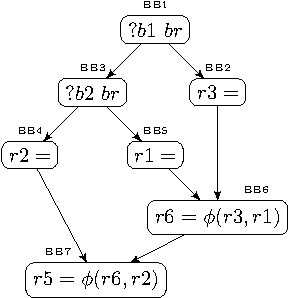
\includegraphics[scale=0.75]{side1}
    \label{fig:side1}}
  \subfloat[After duplication] {
    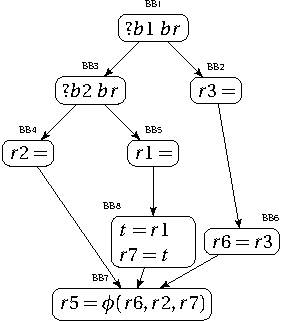
\includegraphics[scale=0.75]{side2}
    \label{fig:side2}}
  \subfloat[sub-region 1] {
    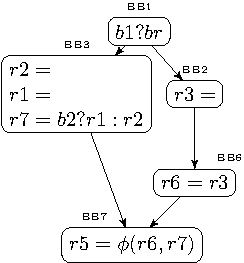
\includegraphics[scale=0.75]{side3}
    \label{fig:side3}}
  \subfloat[sub-region 2] {
    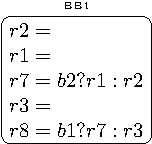
\includegraphics[scale=0.75]{side4}
    \label{fig:side4}}
\caption{Side entry removal using block duplication}
\label{fig:bbdup}
\end{figure}

\section{Global Framework}

Unfortunately, critical regions are rarely composed on simple hammocks or one level nested ifs. Similarly, processors have limited resources. the number of register will determine the acceptable data dependencies, the number of predicate register will determine the depth of the if-conversion. So the ``what'' should help to termine the region to if-convert and the ``how'' the process to optimally compute and place predicates.

The region must be just large enough to have the largest scope of scheduling framework, but in the same time it must not over-commit the machine resources (registers, CPUs). On the contrary, although if-conversion removes branches, I also add some overhead (new instructions to merge predicates, register pressure for speculative conditional, bigger dependence height because of the presence of new data dependencies on the predicates). The newly formed basic block doesn't have a higher schedule estimation than the one that would have been taken if the code was not if-converted.

For this reason, existing approaches of if-conversion are either limited to a single conditional branch using peepholes style of pattern matching, intrinsic functions (conditional code is inlined by the compiler in the internal representation), or scoping larger but restricted regions such as loops hyperblocks. Such approaches require that the region is isolated from the rest of the control flow, , and more important requires a complicated estimation of the future if-converted region. So many factor impact this (predicate computation, register pressure, dependence height) that the objective function needs to be very conservative.

\subsection{Heuristics}

Traditional if-conversion algorithm should be aggressive enough to maximize the use of resource, but should pay attention to:

- Semantic. The merge of different execution path should guarantee that the semantic of the program is preserved
- If-conversion increases register pressure, for two reasons: live ranges are merged and register renaming imposes new constraints
- schedule length: New data dependencies between a predicate definition and it's use, or between a speculated instruction and it's merge, can impede the schedule.

Since the execution cannot use dynamic branch prediction schemes to statically schedule the code, it is essential for the compiler to rely on accurate static branch prediction information \cite{Fisher:1992:PCB:143371.143493}. Using such information, the block selection process can decide whether the inclusion of one path into the other will be beneficial. 

The first consequence is that all registers now live simultaneously, (live range), so the benefits of branch removing and better schedule balanced with increased live range and register pressure : If-conversion must rely on a efficient decision model.

The idea is that a region can be if-converted if the cost of the resulting if-converted basic block is smaller than the cost of each region taken separately weighted by the branch frequencies. The cost of is a factor of 2 parameters:
- resource usage
- schedule length

We compare the ponderated code if the region before if-conversion. So the cost of a path is the schedule estimation of all the blocks in the path ponderated by the probability of execution:
\begin{align}
Cost(path)=Freq(path)*\sum_{k=1}^n(Cost(bb_{k}))
\end{align}
Cost of region starting at basic block $head$ before if-conversion is therefore the cost of all the basic blocks in the considered region, on each paths.
\begin{align}
Cost(head)=Cost(bb_{head})+branch\:lat+Cost(taken\:path)+Cost(fallthu\:path)
\end{align}
One of the path can be empty, in this case only the non empty path will be speculated and it has a zero cost. The Cost after if-conversion is estimated with:
\begin{align}
Cost(head)=Cost(bb_{head} o bb_{taken path} o bb_{fallthru path}) * aggressiveness\:factor
\end{align}

Where $o$ is the composition function that merges basic blocks together, removing associated branches and creating predicate operations. The resulting $Cost$ applied to the new basic block represents the estimated schedule after if-conversion, that will be effective only if $Cost(head_{before\,ifc}) > Cost(head_{after\,ifc})$. This is a conservative algorithm: We don't account for further optimization that will be enabled in the linear code, we have an aggressiveness factor. 
 
The cost function uses the target's machine interface information for instruction's latencies, resources usage and scheduling constraints to estimate the local scheduling. The local dependencies computed between instructions are used to compute the dependence height. The branch frequency is obtained either from static branch prediction heuristics, profile information or user inserted directives.
\begin{figure}
    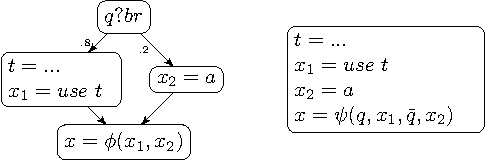
\includegraphics[scale=0.8]{ssa_freq}
\caption{example of profitable if-conversion}
\label{fig:ssa_freq}
\end{figure}

In example \ref{fig:ssa_freq} the dependence height of the fallthru path is 4 cycles. The dependence height of the taken path is 2 cycles. So the ponderated estimated cost of the region is 1+2.4+0.2+1=4.6 cycles. The estimated cost of the if-converted region is the schedule height estimation of the instructions without the branches. In this case, 4 cycles. Since the schedule height of the if-converted region is smaller than the profiled ponderated estimation, then it is profitable.
It should be noted that this heuristic doesn't take into account increased register pressure in the case of speculation, because the variables now interfere. Computing the inteference graph at this stage and simulating a register coalescing process would be extremely expensive at this stage. In the exampe above, a conservative approach would evaluate a register pressure of 4, without counting than $s$ and $t$ coalesce and that in reality the register budget would be 3. Note that this problem is general to every if-conversion algorithm, but might be more easy to deal with in the SSA framework because of the locality of the region.

\subsection{SSA Iterative if-conversion}

Globally, the region to if-convert must be carefully selected. Because of resource consumption issues, merging different paths together can over commit the architecture ability to execute in parallel the multiple instructions: The data dependences and register renaming, introduce new register constraints. Moving operations earlier in the instruction stream increase live-ranges. 
Another pitfall is to increase the critical path by merging long latencies operation from a less frequently executed path, thus moving to the critical paths more instructions than the parallelism could absorb.
Finally, for each basic block considered into the region, a predicate must be computed and assigned to the corresponding instructions. Those predicate computation introduce new instructions and new data dependencies.

Conventional if-conversion algorithm should:

\begin{itemize}
\item Isolate the control flow region for which if-conversion is beneficial, using predictive heuristics. Using tail duplication to remove incoming edges. 
\item then for the whole region, Compute and assign a predicate to each basic block.
\item Convert the instructions into predicated ones using the predicate computed from the basic block, and merge the basic blocks.
\item Apply some predicate reduction mechanism to simplify predicate equations.
\item Finally emit the newly predicate computations and the predicated code. If the ISA is not fully predicated, an additional pass is needed to conditionalize them using conditional moves only.
\end{itemize}

Traditional if-conversion algorithms \cite{Schlansker-predicated} covers those steps separately, so the region is isolated first and then the work is let of the if-conversion algorithm.

In contrast, the SSA iterative based if-conversion  brings together region selection and region transformation, The algorithm is to walk the control flow iteratively 

The algorithm works on a structed directed control flow. Iterates in postorder traversal the list of candidate conditional blocks of the control flow. Postorder traveral garantees that each inner region will be processed before the regions of larger scopes.

The bigger adantage on an incremental optimisation of the control flow is that since nested regions are already predicated when evaluation the if-conversion of a branch, all side effects introduced by the if-conversion, such as new predicate merging instructions, new conditional moves merging flow or new data dependencies will be taken into account. Another advantage is that the predicate assignment is not needed, since new predicates are mechanically inserted when merging inner regions containing conditional code.

The basic region to consider is the Hammock region \cite{Ferrante:1987:PDG:24039.24041}. A Hammock region is a Single Entry Single Exit region. We proposed to a few transformations to convert control flow complex regions into nested Hammocks, such as Basic Block duplication and Predicate merging. The prevalent idea is that inner region once predicated will be viewed as a single basic region by the outer scopes.

Consider for example the control flow transformations for the $wc$ program (figure \ref{fig:wc1}).
(The formation of conditional instructions will be detailed in the next section).
 The postorder list of the basic nested regions is {\em BB11, BB17, BB16, BB14, BB10, BB9, BB6, BB2} (The start of the nested regions are represented by the circle nodes). First, for BB11, BB12 is promoted and BB2 becomes a fall-thru of BB11 . For the region starting at BB17, BB19 cannot be promoted because of the side entry coming from BB15. BB16 is the start of a logical region from the two predicates BB16 BB17. A new predicate is computed from the one defined in BB17 and the one defined in BB16. BB17 is promoted and the registers alive in BB19 are conditionalized with the new predicate. The process continues on BB16. BB19 is duplicated to remove the side edge. BB14 is the head of the newly created region where BB15, BB16 and BB17 can be promoted. From BB9 a logif predicate is computed with the one in BB10. Instructions in BB14 are conditionalized on this new predicate and BB10 promoted, forming a new hammock at BB9 with BB14 and BB11 that can be promoted. The last candidate, BB2 is the start of a region that cannot be promoted, because of the call into BB3. the region is if-converted, leaving a single back-edge, removing 7 branches inside the body loop.

\begin{figure}
  \subfloat[Before if-conversion] {
    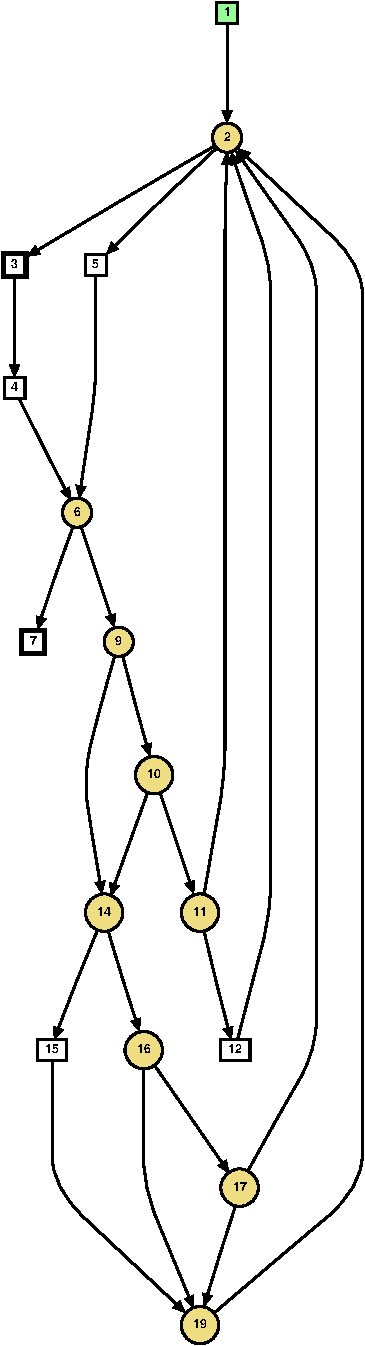
\includegraphics[scale=0.6]{graph1}
    \label{fig:wc1}}
  \subfloat[After if-conversion] {
    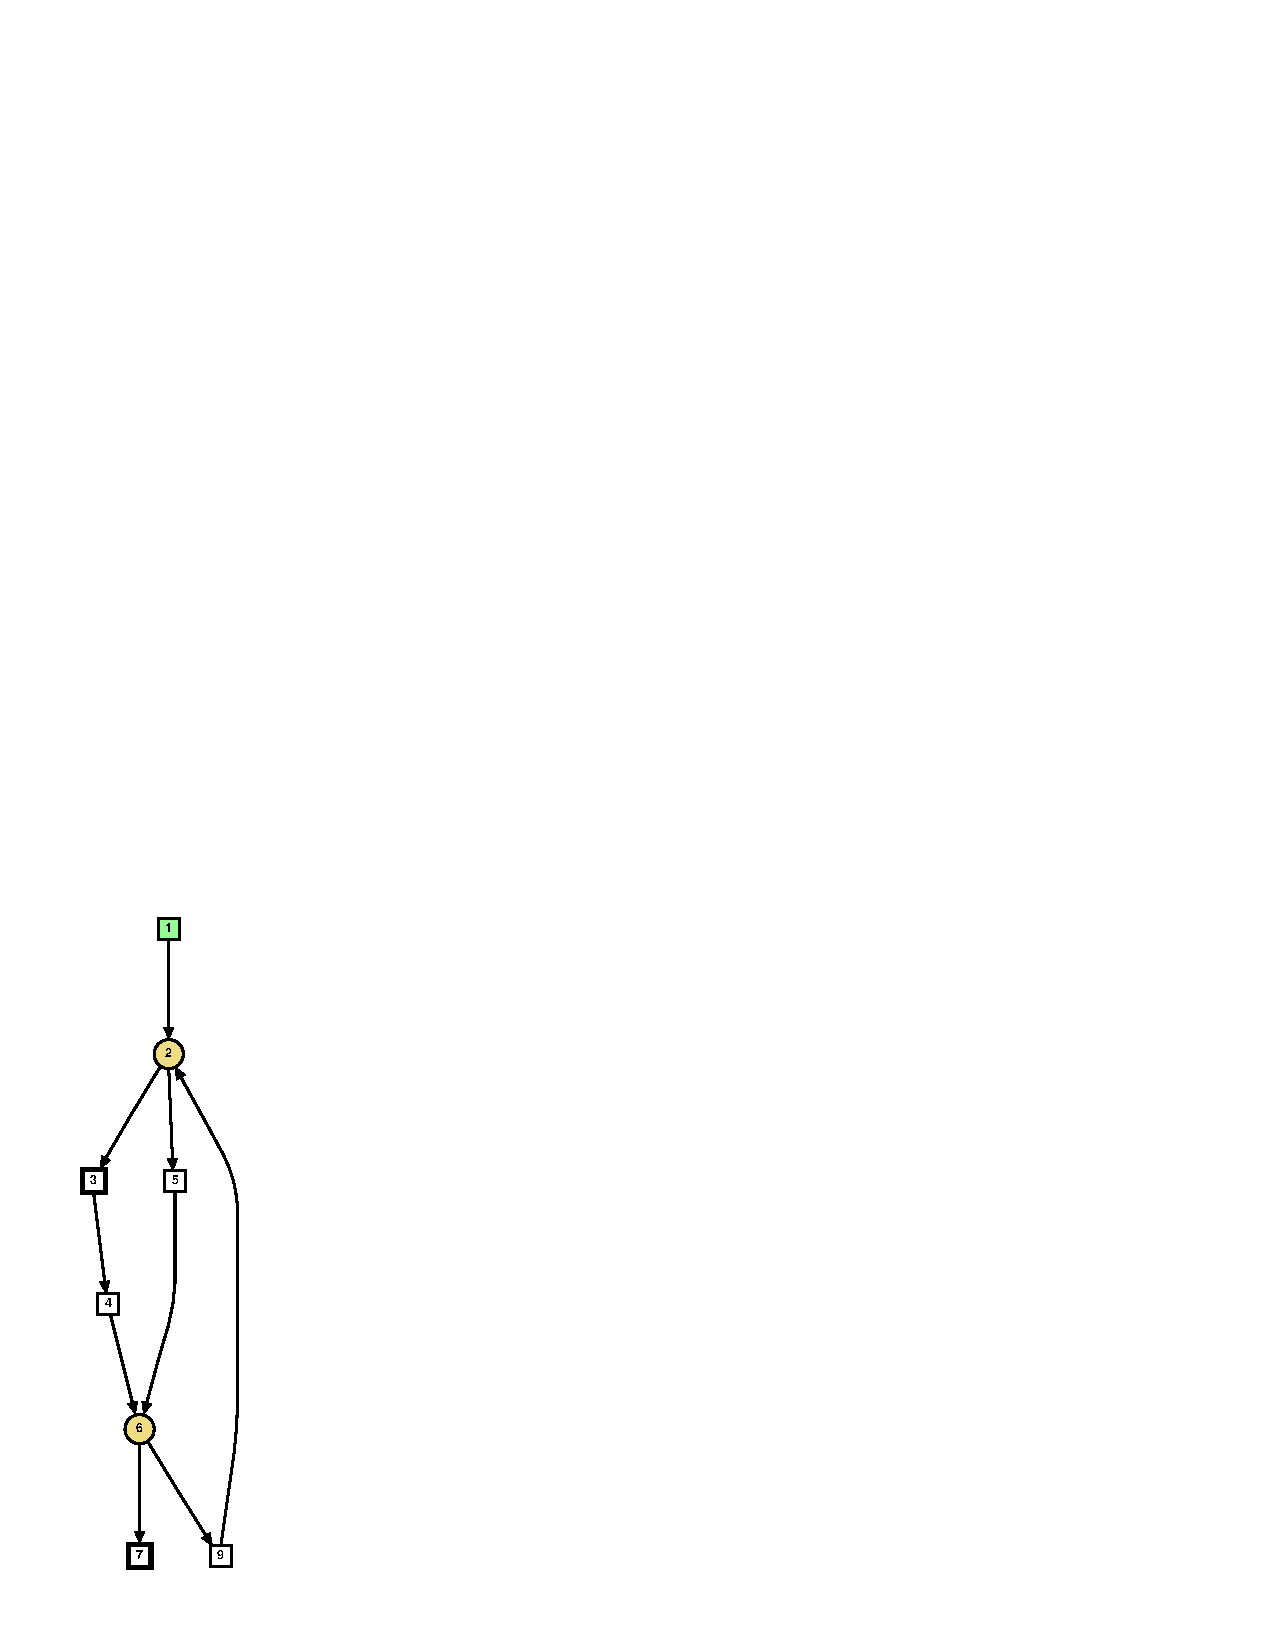
\includegraphics[scale=0.6]{graph7}
    \label{fig:wc2}}
\label{fig:wc example}
\end{figure}

All those operations make the if-conversion process a complex optimization, forcing designers to be extremely conservative, as the objective functions must contain variables not known at the start of the transformation. (such as the complexity of the predicate equations) since moving multiple control paths together can easily exceed processors resources (leading to excessive register pressure) or move infrequently used expensive instruction (memory loads) into the critical path. 

Set of transformations are applied iteratively and aggressively in postorder of the CFG
Start from first inner regions of basic blocks with a single conditional entry
Blocks reached on multiple conditions are detected (predicate merge)
Side entries removed using block duplication 
Decision to continue reconsidered for each region. ``The whole doesn't' exeed the sum of the parts''' or when hazardous instructions

\subsection{Hyperblocks}

Traditional framework of if-conversion use Hyperblocks as the basic predicated region formation. \cite{Mahlke:1992:ECS:144965.144998}. A hyper block is a region of code with a single entry and possible, multiple exits where inner branches have been removed thru if-conversion. Tail duplication is used to exclude from the Hyperblock basic blocks, either because the contain hazardous instructions, or because heuristic decision. 
Traditional hyperblocks formation algorithm create the hyperblocks in the following steps:
\begin{itemize}
\item Create a trace and block selection. A trace is a sequence of basic blocks that can be scheduled together. 
\item Remove side entries with tail duplication, This steps removes scheduling constraints imposed by side entries, or allow regions to be if-converted despite hazards.
\item Finally, if-conversion can be performed to form the hyperblock. 
\end{itemize}

As an example of hyperblock formation, consider the example \ref{fig:hyper1}. This loop contains two branches, and so if-converting it would be profitable. However, block selection has excluded BB2. and had integrated BB5, because heuristics have determined that the schedule of BB5 inside BB4 would be beneficial. The hyperblock contains {BB1, BB3, BB4, BB5, BB6}. Since BB4 is has side entry, it must be removed by tail duplication. \ref{fig:hyper2} shows the  control flow after block duplication. Notice that a new node, BB7, have been added after the tail duplication by a process called branch coalescing. Finally \ref{fig:hyper3} shows the code once if-converted.

\begin{figure}[h]
  \subfloat[loop] {
    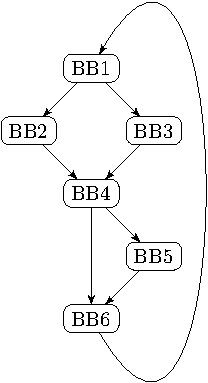
\includegraphics[scale=0.7]{hyper1}
    \label{fig:hyper1}}
  \subfloat[standard tail-duplication] {
    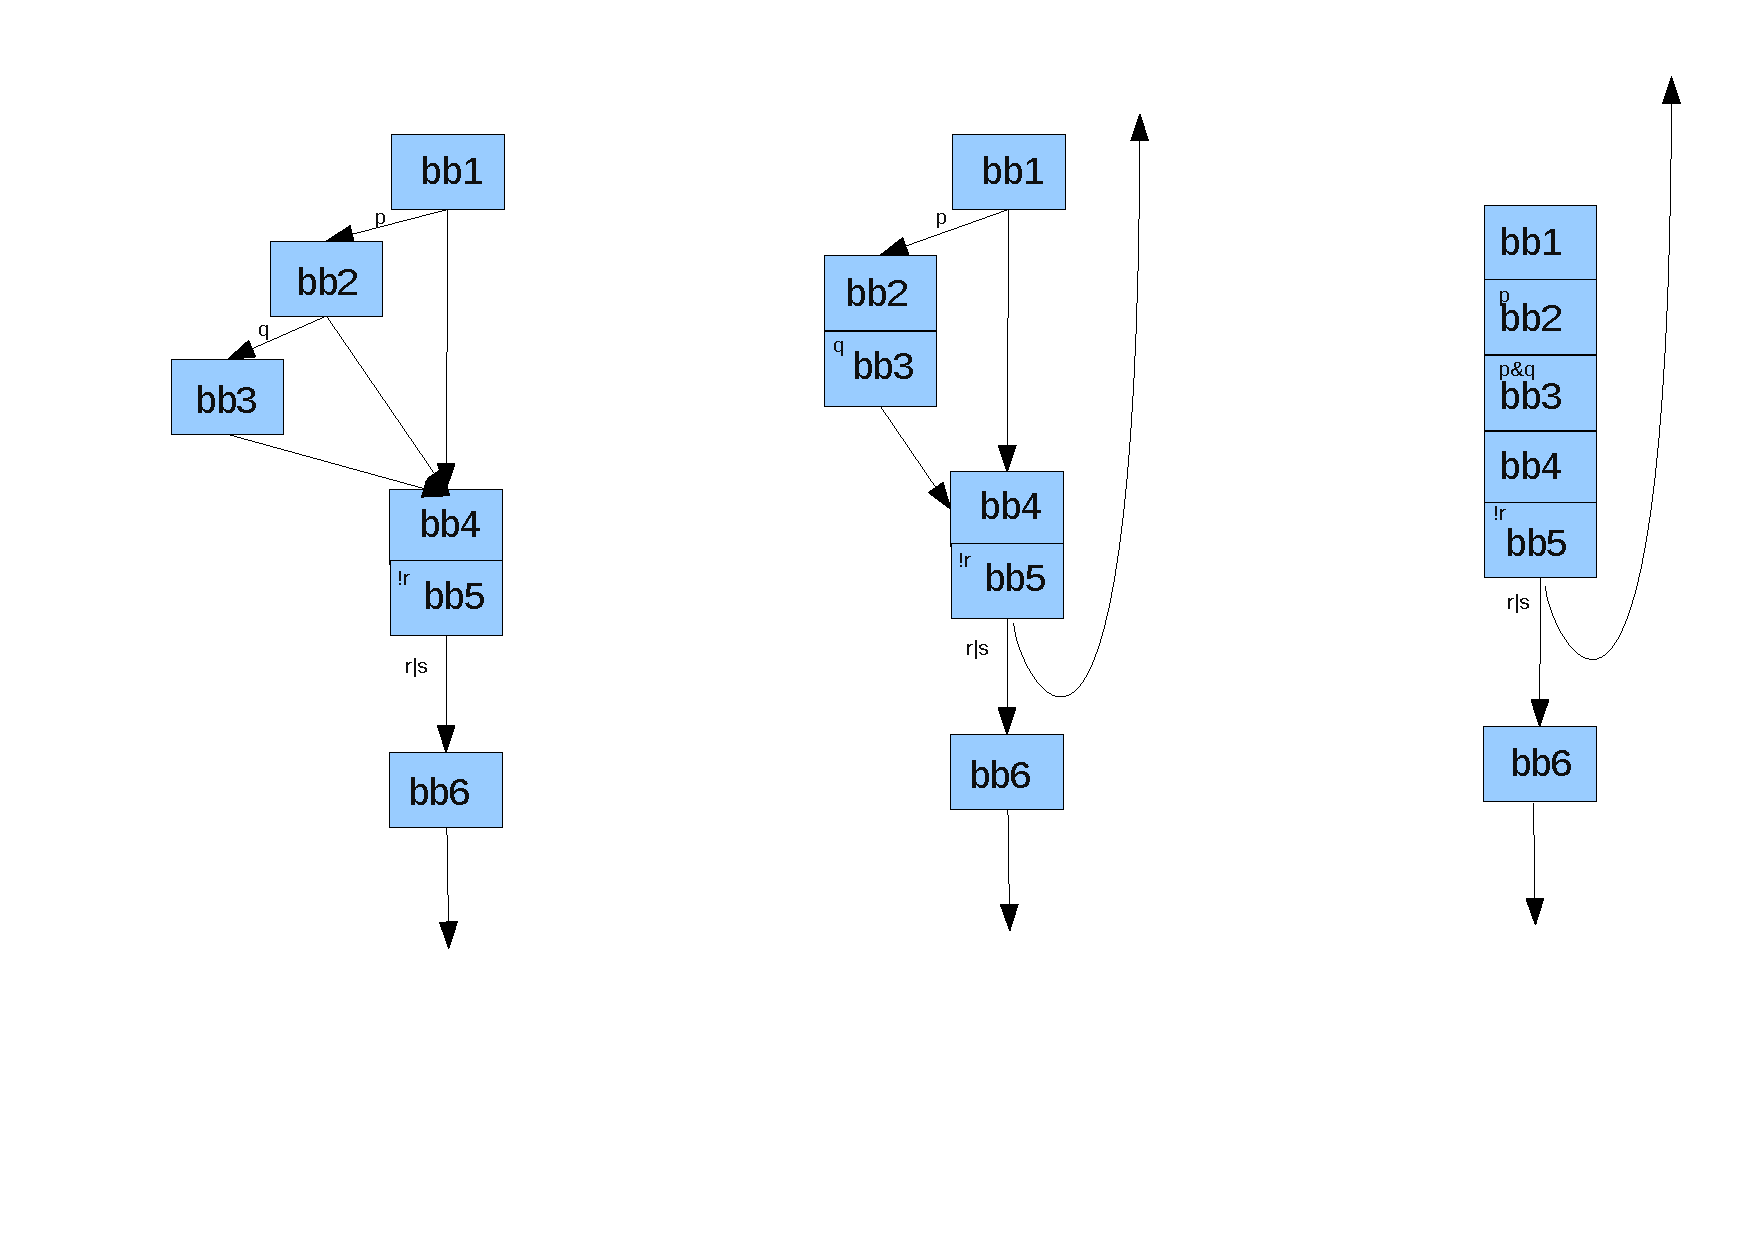
\includegraphics[scale=0.7]{hyper2}
    \label{fig:hyper2}}
  \subfloat[after SSA if-conversion] {
    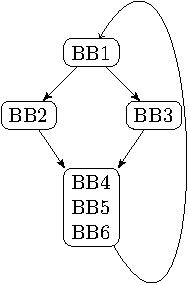
\includegraphics[scale=0.7]{hyper4}
    \label{fig:hyper4}}
  \subfloat[final flow] {
    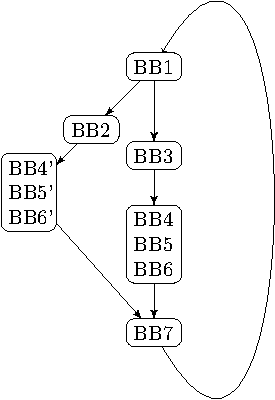
\includegraphics[scale=0.7]{hyper3}
    \label{fig:hyper3}}
\end{figure}

The fact that the if-conversion happens after tail-duplication. In the resulting code happens to be difficult to schedule efficiently, over committing resources. Hyperblock formation, if-conversion and speculation introduce a major phase ordering problem. A technique called ``Reverse If-Conversion'' \cite{August:1999:PRI:326224.325595} overcomes this problem, allowing to use aggressive if-conversion framework and reconstructing the control flow at schedule time.

Consider in contrast how tail-duplication is performed in a lazy way, after the code have been if-converted. \ref{fig:hyper4} shows the same loop body were the second $if$ region have been SSA if-converted. The decision to if-convert the region formed by {BB1, BB2, BB3} is now local and can be taken conservatively. Only at this stage, if necessary, tail-duplication can be performed to remove the side entry coming from BB2. Duplicating a single predicated block is now a very simple operation.

\section{Conclusion} 
We presented in this chapter a novel if-conversion algorithm that takes advantage of the SSA properties to efficiency assign predicates and layout the new control flow in an iterative, bottom up process. As opposed to the other top-down approach, this algorithm is very conservative, since the benefit of if-conversion is reevaluated at each nested transformation.
We show that we reunified region-formation and if-conversion in a single process, hyperblocks being created lazily, using well known techniques such as tail-duplication or branch coalescing only when the benefits is established.
Predication and speculation are often presented as two different alternatives for if-conversion. While it is true than they both require different hardware support, they should coexist in an efficient if-conversion process so every model of conditional execution is accepted. Thanks to conditional moves and $\psi$ transformations, they are now generated together in the same framework. The algorithm was proven to be efficient in real world context. For example, polynomial evaluation, for which specific ILP algorithm are designed can be fully if-converted in a straight-line of code \cite{JeKnMoRe11}, or we measured speedups up to 30\% on linux-scalar (spec benchs)  or embedded (eembc) application, without code size penalty.







	% \printindex
	\bibliographystyle{plain}
	\bibliography{../../book}

\end{document}
